\documentclass[]{article}
\usepackage{lmodern}
\usepackage{amssymb,amsmath}
\usepackage{ifxetex,ifluatex}
\usepackage{fixltx2e} % provides \textsubscript
\ifnum 0\ifxetex 1\fi\ifluatex 1\fi=0 % if pdftex
  \usepackage[T1]{fontenc}
  \usepackage[utf8]{inputenc}
\else % if luatex or xelatex
  \ifxetex
    \usepackage{mathspec}
  \else
    \usepackage{fontspec}
  \fi
  \defaultfontfeatures{Ligatures=TeX,Scale=MatchLowercase}
  \newcommand{\euro}{€}
\fi
% use upquote if available, for straight quotes in verbatim environments
\IfFileExists{upquote.sty}{\usepackage{upquote}}{}
% use microtype if available
\IfFileExists{microtype.sty}{%
\usepackage{microtype}
\UseMicrotypeSet[protrusion]{basicmath} % disable protrusion for tt fonts
}{}
\usepackage[margin=1in]{geometry}
\usepackage{hyperref}
\PassOptionsToPackage{usenames,dvipsnames}{color} % color is loaded by hyperref
\hypersetup{unicode=true,
            pdftitle={rfPermute: Estimation of predictor importance significance in Random Forest models},
            pdfauthor={Frederick I. Archer},
            pdfborder={0 0 0},
            breaklinks=true}
\urlstyle{same}  % don't use monospace font for urls
\usepackage{color}
\usepackage{fancyvrb}
\newcommand{\VerbBar}{|}
\newcommand{\VERB}{\Verb[commandchars=\\\{\}]}
\DefineVerbatimEnvironment{Highlighting}{Verbatim}{commandchars=\\\{\}}
% Add ',fontsize=\small' for more characters per line
\usepackage{framed}
\definecolor{shadecolor}{RGB}{248,248,248}
\newenvironment{Shaded}{\begin{snugshade}}{\end{snugshade}}
\newcommand{\KeywordTok}[1]{\textcolor[rgb]{0.13,0.29,0.53}{\textbf{{#1}}}}
\newcommand{\DataTypeTok}[1]{\textcolor[rgb]{0.13,0.29,0.53}{{#1}}}
\newcommand{\DecValTok}[1]{\textcolor[rgb]{0.00,0.00,0.81}{{#1}}}
\newcommand{\BaseNTok}[1]{\textcolor[rgb]{0.00,0.00,0.81}{{#1}}}
\newcommand{\FloatTok}[1]{\textcolor[rgb]{0.00,0.00,0.81}{{#1}}}
\newcommand{\ConstantTok}[1]{\textcolor[rgb]{0.00,0.00,0.00}{{#1}}}
\newcommand{\CharTok}[1]{\textcolor[rgb]{0.31,0.60,0.02}{{#1}}}
\newcommand{\SpecialCharTok}[1]{\textcolor[rgb]{0.00,0.00,0.00}{{#1}}}
\newcommand{\StringTok}[1]{\textcolor[rgb]{0.31,0.60,0.02}{{#1}}}
\newcommand{\VerbatimStringTok}[1]{\textcolor[rgb]{0.31,0.60,0.02}{{#1}}}
\newcommand{\SpecialStringTok}[1]{\textcolor[rgb]{0.31,0.60,0.02}{{#1}}}
\newcommand{\ImportTok}[1]{{#1}}
\newcommand{\CommentTok}[1]{\textcolor[rgb]{0.56,0.35,0.01}{\textit{{#1}}}}
\newcommand{\DocumentationTok}[1]{\textcolor[rgb]{0.56,0.35,0.01}{\textbf{\textit{{#1}}}}}
\newcommand{\AnnotationTok}[1]{\textcolor[rgb]{0.56,0.35,0.01}{\textbf{\textit{{#1}}}}}
\newcommand{\CommentVarTok}[1]{\textcolor[rgb]{0.56,0.35,0.01}{\textbf{\textit{{#1}}}}}
\newcommand{\OtherTok}[1]{\textcolor[rgb]{0.56,0.35,0.01}{{#1}}}
\newcommand{\FunctionTok}[1]{\textcolor[rgb]{0.00,0.00,0.00}{{#1}}}
\newcommand{\VariableTok}[1]{\textcolor[rgb]{0.00,0.00,0.00}{{#1}}}
\newcommand{\ControlFlowTok}[1]{\textcolor[rgb]{0.13,0.29,0.53}{\textbf{{#1}}}}
\newcommand{\OperatorTok}[1]{\textcolor[rgb]{0.81,0.36,0.00}{\textbf{{#1}}}}
\newcommand{\BuiltInTok}[1]{{#1}}
\newcommand{\ExtensionTok}[1]{{#1}}
\newcommand{\PreprocessorTok}[1]{\textcolor[rgb]{0.56,0.35,0.01}{\textit{{#1}}}}
\newcommand{\AttributeTok}[1]{\textcolor[rgb]{0.77,0.63,0.00}{{#1}}}
\newcommand{\RegionMarkerTok}[1]{{#1}}
\newcommand{\InformationTok}[1]{\textcolor[rgb]{0.56,0.35,0.01}{\textbf{\textit{{#1}}}}}
\newcommand{\WarningTok}[1]{\textcolor[rgb]{0.56,0.35,0.01}{\textbf{\textit{{#1}}}}}
\newcommand{\AlertTok}[1]{\textcolor[rgb]{0.94,0.16,0.16}{{#1}}}
\newcommand{\ErrorTok}[1]{\textcolor[rgb]{0.64,0.00,0.00}{\textbf{{#1}}}}
\newcommand{\NormalTok}[1]{{#1}}
\usepackage{graphicx,grffile}
\makeatletter
\def\maxwidth{\ifdim\Gin@nat@width>\linewidth\linewidth\else\Gin@nat@width\fi}
\def\maxheight{\ifdim\Gin@nat@height>\textheight\textheight\else\Gin@nat@height\fi}
\makeatother
% Scale images if necessary, so that they will not overflow the page
% margins by default, and it is still possible to overwrite the defaults
% using explicit options in \includegraphics[width, height, ...]{}
\setkeys{Gin}{width=\maxwidth,height=\maxheight,keepaspectratio}
\setlength{\parindent}{0pt}
\setlength{\parskip}{6pt plus 2pt minus 1pt}
\setlength{\emergencystretch}{3em}  % prevent overfull lines
\providecommand{\tightlist}{%
  \setlength{\itemsep}{0pt}\setlength{\parskip}{0pt}}
\setcounter{secnumdepth}{0}

%%% Use protect on footnotes to avoid problems with footnotes in titles
\let\rmarkdownfootnote\footnote%
\def\footnote{\protect\rmarkdownfootnote}

%%% Change title format to be more compact
\usepackage{titling}

% Create subtitle command for use in maketitle
\newcommand{\subtitle}[1]{
  \posttitle{
    \begin{center}\large#1\end{center}
    }
}

\setlength{\droptitle}{-2em}
  \title{rfPermute: Estimation of predictor importance significance in Random
Forest models}
  \pretitle{\vspace{\droptitle}\centering\huge}
  \posttitle{\par}
  \author{Frederick I. Archer}
  \preauthor{\centering\large\emph}
  \postauthor{\par}
  \date{}
  \predate{}\postdate{}



% Redefines (sub)paragraphs to behave more like sections
\ifx\paragraph\undefined\else
\let\oldparagraph\paragraph
\renewcommand{\paragraph}[1]{\oldparagraph{#1}\mbox{}}
\fi
\ifx\subparagraph\undefined\else
\let\oldsubparagraph\subparagraph
\renewcommand{\subparagraph}[1]{\oldsubparagraph{#1}\mbox{}}
\fi

\begin{document}
\maketitle

\subsection{Abstract}\label{abstract}

One of the strengths of the ensemble machine learning algorithm, Random
Forest, is its ability to estimate the relative importance of predictors
within classification and regression models. However, there is no method
for identifying which predictors are significantly more important than
what would be expected by random chance. I present the \emph{rfPermute}
package which is a wrapper for the commonly used \emph{randomForest}
package that produces permutation-based estimates of predictor
importance significance. The package also includes utility functions for
summarizing and visualizing Random Forest model results.

\subsection{Introduction}\label{introduction}

Since its inception, the ensemble machine learning algorithm, Random
Forest (Breiman 2001), has been rapidly gaining popularity as a powerful
tool for classification and uncovering patterns in complex data sets.
Because it is non-parametric and produces internally-validated
classification models, it has been used in a wide variety of fields (D.
R. Cutler et al. 2007; Touw et al. 2012; Winham et al. 2012), and has
proven to be robust in performance tests against other commonly used
modelling algorithms (Berk 2006).

The most common implementation of Random Forest is the
\emph{randomForest} package (Liaw and Wiener 2002). This package allows
easy specification of both classification and regression models and
provides several useful functions for summarizing their results. One of
the metrics that many users of Random Forest are interested in examining
are the measures of variable or predictor importance. The importance of
a predictor is estimated by measuring the decrease in prediction
accuracy when that predictor is permuted in each tree in the forest.
These values are often used to identify and rank those predictors that
are most related to the response and critical for classification. More
detail about how the various importance metrics are computed can be
found in Breiman (2002), Liaw and Wiener (2002), as well as the help
file for the \texttt{importance} function in \emph{randomForest}.\\
However, \emph{randomForest} only produces raw measures of predictor
importance and it is up to the user to identify cutoff values above
which predictors would be considered to have a significant impact on
model predictions. In order to address this, I have implemented a
permutation test called \emph{rfPermute} which generates a null
distribution of importance scores for each predictor against which the
observed importance scores are compared. This null distribution is
created by randomly permuting the response variable (class assignments
in a classification model, or independent continuous response in a
regression model) among cases, running the same Random Forest model on
the permuted data, and storing the resulting importance scores.

Under this procedure, a predictor that is not adding any significant
information to the model will have an observed importance score that is
similar to those generated by a random shuffling of the response, while
a significant predictor will have an importance score much larger than
the null. Significance p-values are then calculated as the fraction of
replicates in the null distribution that are greater than or equal to
the observed value. \emph{rfPermute} provides both the p-values and the
null distribution which the user can use for variable selection and
further exploration.

\subsection{Execution}\label{execution}

The function, \texttt{rfPermute}, provides a wrapper for the
\texttt{randomForest} function that accepts all of its arguments, plus
two additional ones: \texttt{nrep}, which is an integer specifying the
number of permutation replicates to run, and \texttt{num.cores}, which
is an integer specifying the number of CPU cores to distribute the
permutations over on a multi-core system. If \texttt{nrep} is set to 0,
then the return value is a list with the same elements as the equivalent
call to \texttt{randomForest}. With one or more permutation replicates
specified, the returned list contains two elements: \texttt{null.dist},
which is a list containing arrays of the null distributions for unscaled
and scaled importance measures, and \texttt{pval}, which is an array
containing the permutation p-values for unscaled and scaled importance
measures.

As an example, we use \texttt{rfPermute} to create a classifier of four
clades of the endosymbiont dinoflagellate \emph{Symbiodinium} from a
data set of metabolite profiles as published in Klueter et al (2015).
Significance is measured with 1000 permutations. Because each
\emph{Symbiodinium} type is represented by 16 cases in this data set, we
create a model where 8 cases from each type are used in each tree, and
sampling is done without replacement. This scheme ensures that in each
tree, half of the samples from each class are used for trainng, while
the other half are retained as out-of-bag (OOB) for testing.
\texttt{rfPermute} automatically sets \texttt{importance\ =\ TRUE} to
force \texttt{randomForest} to calculate and return the matrix of
importance scores, so we don't need to set that. However, we will be
using the proximity matrix later, so we must specify
\texttt{proximity\ =\ TRUE}.

\begin{Shaded}
\begin{Highlighting}[]
\CommentTok{# Load the package}
\KeywordTok{library}\NormalTok{(rfPermute)}
\end{Highlighting}
\end{Shaded}

\begin{Shaded}
\begin{Highlighting}[]
\CommentTok{# Load the metabolomics data set}
\KeywordTok{data}\NormalTok{(symb.metab)}

\CommentTok{# Create the randomForest model with 1000}
\CommentTok{# permutations.}
\NormalTok{metab.rf <-}\StringTok{ }\KeywordTok{rfPermute}\NormalTok{(type ~}\StringTok{ }\NormalTok{., }\DataTypeTok{data =} \NormalTok{symb.metab, }
    \DataTypeTok{sampsize =} \KeywordTok{rep}\NormalTok{(}\DecValTok{8}\NormalTok{, }\DecValTok{4}\NormalTok{), }\DataTypeTok{replace =} \OtherTok{FALSE}\NormalTok{, }\DataTypeTok{proximity =} \OtherTok{TRUE}\NormalTok{, }
    \DataTypeTok{nrep =} \DecValTok{1000}\NormalTok{)}
\NormalTok{metab.rf}
\end{Highlighting}
\end{Shaded}

\begin{verbatim}

Call:
 randomForest(formula = type ~ ., data = symb.metab, sampsize = rep(8,      4), replace = FALSE, proximity = TRUE) 
               Type of random forest: classification
                     Number of trees: 500
No. of variables tried at each split: 12

        OOB estimate of  error rate: 3.12%
Confusion matrix:
     A194 B184 B224 D206 class.error
A194   15    0    0    1      0.0625
B184    0   16    0    0      0.0000
B224    0    0   15    1      0.0625
D206    0    0    0   16      0.0000
\end{verbatim}

The result is a \texttt{rfPermute} object that inherits from and has the
same components as a \texttt{randomForest} object, plus
\texttt{null.dist} and \texttt{pval}, as seen below.

\begin{Shaded}
\begin{Highlighting}[]
\KeywordTok{class}\NormalTok{(metab.rf)}
\end{Highlighting}
\end{Shaded}

\begin{verbatim}
[1] "rfPermute"            "randomForest.formula"
[3] "randomForest"        
\end{verbatim}

\begin{Shaded}
\begin{Highlighting}[]
\KeywordTok{names}\NormalTok{(metab.rf)}
\end{Highlighting}
\end{Shaded}

\begin{verbatim}
 [1] "call"            "type"           
 [3] "predicted"       "err.rate"       
 [5] "confusion"       "votes"          
 [7] "oob.times"       "classes"        
 [9] "importance"      "importanceSD"   
[11] "localImportance" "proximity"      
[13] "ntree"           "mtry"           
[15] "forest"          "y"              
[17] "test"            "inbag"          
[19] "null.dist"       "pval"           
[21] "terms"          
\end{verbatim}

\begin{Shaded}
\begin{Highlighting}[]
\KeywordTok{str}\NormalTok{(metab.rf$null.dist)}
\end{Highlighting}
\end{Shaded}

\begin{verbatim}
List of 2
 $ unscaled: num [1:155, 1:6, 1:1000] 0.0015 0.0005 -0.0015 0.00075 0.0005 -0.001 -0.00025 -0.00025 -0.0005 -0.002 ...
  ..- attr(*, "dimnames")=List of 3
  .. ..$ : chr [1:155] "Amino.Acid.2" "Amino.Acid.3" "Alanine" "Amino.Acid.4" ...
  .. ..$ : chr [1:6] "A194" "B184" "B224" "D206" ...
  .. ..$ : NULL
 $ scaled  : num [1:155, 1:6, 1:1000] 1.904 0.707 -2.131 0.6 0.447 ...
  ..- attr(*, "dimnames")=List of 3
  .. ..$ : chr [1:155] "Amino.Acid.2" "Amino.Acid.3" "Alanine" "Amino.Acid.4" ...
  .. ..$ : chr [1:6] "A194" "B184" "B224" "D206" ...
  .. ..$ : NULL
\end{verbatim}

\begin{Shaded}
\begin{Highlighting}[]
\KeywordTok{str}\NormalTok{(metab.rf$pval)}
\end{Highlighting}
\end{Shaded}

\begin{verbatim}
 num [1:155, 1:6, 1:2] 0.3367 0.3966 0.4236 0.0889 0.4565 ...
 - attr(*, "dimnames")=List of 3
  ..$ : chr [1:155] "Amino.Acid.2" "Amino.Acid.3" "Alanine" "Amino.Acid.4" ...
  ..$ : chr [1:6] "A194" "B184" "B224" "D206" ...
  ..$ : chr [1:2] "unscaled" "scaled"
\end{verbatim}

\subsection{Predictor significance}\label{predictor-significance}

The permutation p-values for predictors in the \texttt{rfPermute} object
can be accessed using the \texttt{rp.importance} function, which behaves
in the same manner as \texttt{randomForest::importance}, returning a
matrix of the scaled or unscaled importance scores along with their
respective p-values.

\begin{Shaded}
\begin{Highlighting}[]
\NormalTok{imp <-}\StringTok{ }\KeywordTok{rp.importance}\NormalTok{(metab.rf)}
\KeywordTok{head}\NormalTok{(imp)}
\end{Highlighting}
\end{Shaded}

\begin{verbatim}
                      A194   A194.pval     B184
C30..5.Sterol     8.509105 0.000999001 9.654092
C28..5.Sterol    10.479585 0.000999001 7.310758
C29.Stanol.2      6.641183 0.000999001 6.692812
Sugar.17          5.561427 0.000999001 5.001033
Closed.Hexose.5   8.138557 0.000999001 6.961631
C28..5.22.Sterol  4.478776 0.001998002 5.730685
                   B184.pval     B224   B224.pval
C30..5.Sterol    0.000999001 6.915300 0.000999001
C28..5.Sterol    0.000999001 6.224220 0.000999001
C29.Stanol.2     0.000999001 5.111778 0.000999001
Sugar.17         0.000999001 7.952449 0.000999001
Closed.Hexose.5  0.000999001 3.903217 0.004995005
C28..5.22.Sterol 0.000999001 4.669289 0.000999001
                      D206   D206.pval
C30..5.Sterol    10.241161 0.000999001
C28..5.Sterol     6.088147 0.000999001
C29.Stanol.2      9.461333 0.000999001
Sugar.17          6.903033 0.000999001
Closed.Hexose.5   3.289976 0.005994006
C28..5.22.Sterol  6.873986 0.000999001
                 MeanDecreaseAccuracy
C30..5.Sterol               11.049444
C28..5.Sterol               10.447258
C29.Stanol.2                 9.730202
Sugar.17                     8.655595
Closed.Hexose.5              8.629144
C28..5.22.Sterol             7.689850
                 MeanDecreaseAccuracy.pval
C30..5.Sterol                  0.000999001
C28..5.Sterol                  0.000999001
C29.Stanol.2                   0.000999001
Sugar.17                       0.000999001
Closed.Hexose.5                0.000999001
C28..5.22.Sterol               0.000999001
                 MeanDecreaseGini
C30..5.Sterol           1.5155494
C28..5.Sterol           1.3630128
C29.Stanol.2            1.1727002
Sugar.17                1.1421368
Closed.Hexose.5         0.8792825
C28..5.22.Sterol        0.7644224
                 MeanDecreaseGini.pval
C30..5.Sterol              0.000999001
C28..5.Sterol              0.000999001
C29.Stanol.2               0.000999001
Sugar.17                   0.000999001
Closed.Hexose.5            0.000999001
C28..5.22.Sterol           0.000999001
\end{verbatim}

A density plot of the null distribution of predictor importances along
with the observed importance value can be visulized with the
\texttt{plotNull} function (Fig. 1).

\begin{Shaded}
\begin{Highlighting}[]
\KeywordTok{plotNull}\NormalTok{(metab.rf, }\DataTypeTok{preds =} \StringTok{"Disaccharide.8"}\NormalTok{, }\DataTypeTok{imp.type =} \StringTok{"MeanDecreaseAccuracy"}\NormalTok{)}
\end{Highlighting}
\end{Shaded}

\begin{figure}[htbp]
\centering
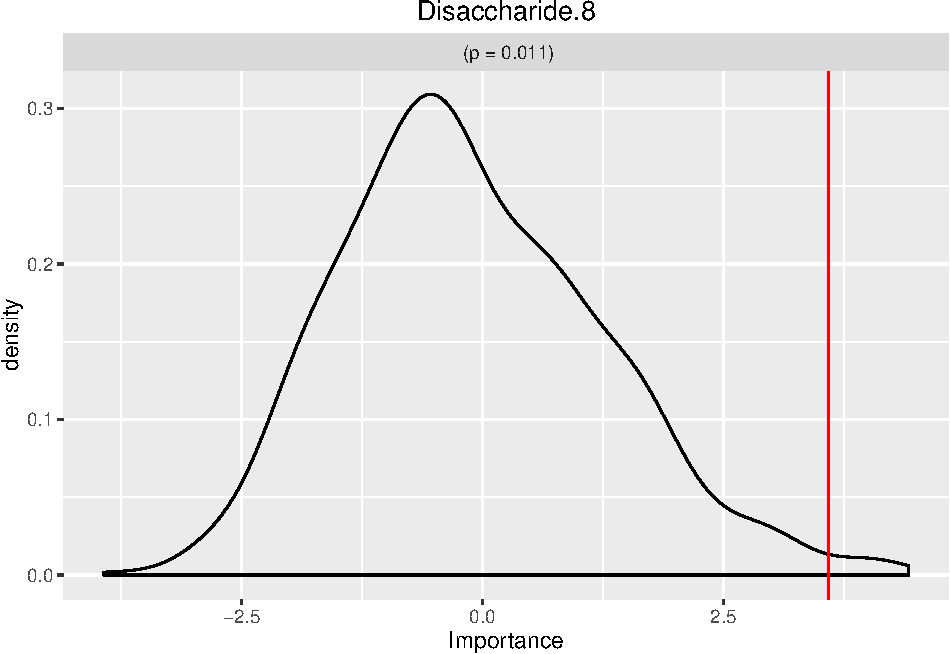
\includegraphics{rfPermute_ms_files/figure-latex/plotNull-1.pdf}
\caption{Null distribution of mean decrease in accuracy for the
predictor metabolite, `Disaccharide.8'.}
\end{figure}

An ordered bar chart of all predictor importances with designations of
their significance at a specified critical \(\alpha\) (traditionally
0.05), can be visualized with the \texttt{plot} function applied to the
result of \texttt{rp.importance}. Figure 2 shows that approximately the
top third of the predictor metabolites are deemed significant at p
\textless{}= 0.05, even though the distributon of importance scores
shows a steady decline with no obvious break in this region.

\begin{Shaded}
\begin{Highlighting}[]
\KeywordTok{plot}\NormalTok{(imp, }\DataTypeTok{type =} \StringTok{"MeanDecreaseAccuracy"}\NormalTok{)}
\end{Highlighting}
\end{Shaded}

\begin{figure}[htbp]
\centering
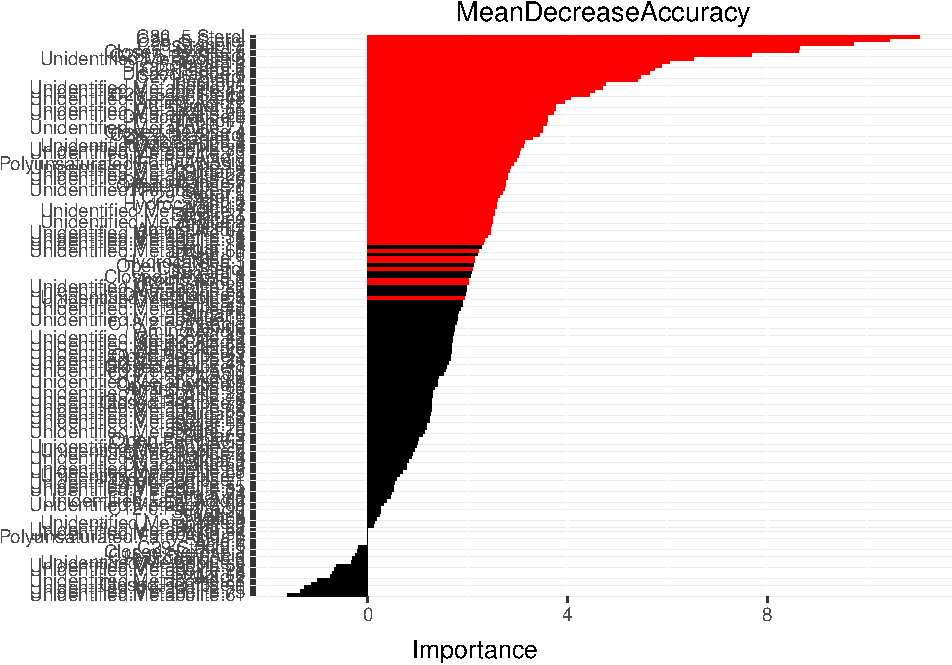
\includegraphics{rfPermute_ms_files/figure-latex/plot_imp1-1.pdf}
\caption{Bar chart of mean decrease in accuracy. Bars colored in red
have p-values \textless{}= 0.05.}
\end{figure}

Given that we can't see much detail about specific predictor
metabolites, we can also show just the top 10 most important predictors,
but this time for all importance types (Fig. 3). The figure can also be
restricted to show only significant predictors by specifying
\texttt{sig.only\ =\ TRUE} to the \texttt{plot} function.

\begin{Shaded}
\begin{Highlighting}[]
\KeywordTok{plot}\NormalTok{(imp, }\DataTypeTok{n =} \DecValTok{10}\NormalTok{)}
\end{Highlighting}
\end{Shaded}

\begin{figure}[htbp]
\centering
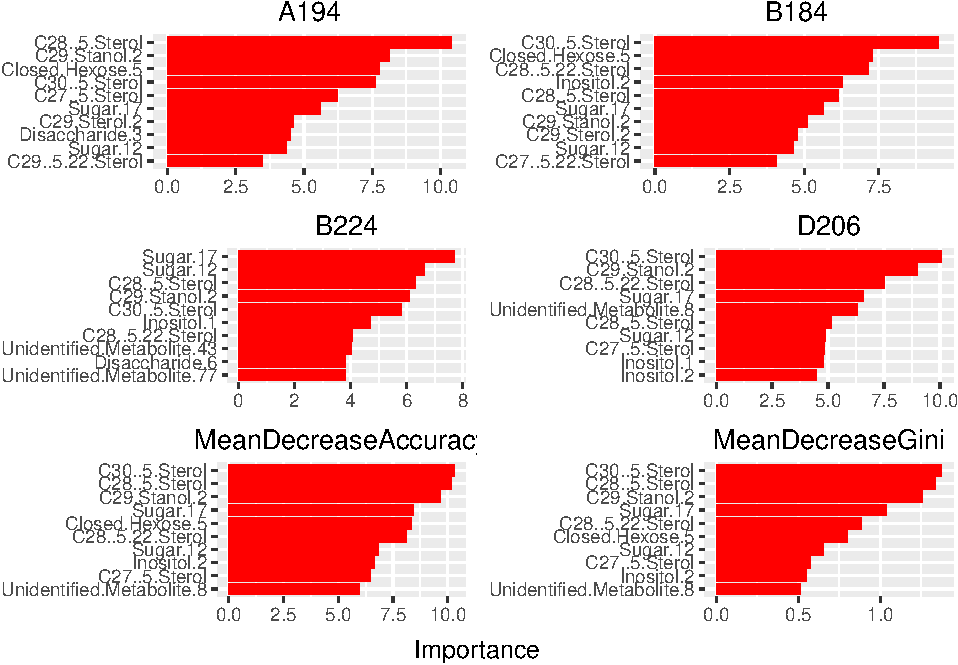
\includegraphics{rfPermute_ms_files/figure-latex/plot_imp2-1.pdf}
\caption{Bar chart of top ten most important predictors.}
\end{figure}

Figure 3 shows that many of the same metabolites are significantly
important for all classes. To better visualize the relative distribution
of predictor importance across classes we can also produce a heatmap
(Fig. 4). Although many of the same metabolites rank high for all
classes, there are several lower down in the list that are significant
in some classes, but not in others, suggesting that they have strong
diagnostic properties for those subsets of classes.

\begin{Shaded}
\begin{Highlighting}[]
\KeywordTok{impHeatmap}\NormalTok{(metab.rf, }\DataTypeTok{n =} \DecValTok{30}\NormalTok{)}
\end{Highlighting}
\end{Shaded}

\begin{figure}[htbp]
\centering
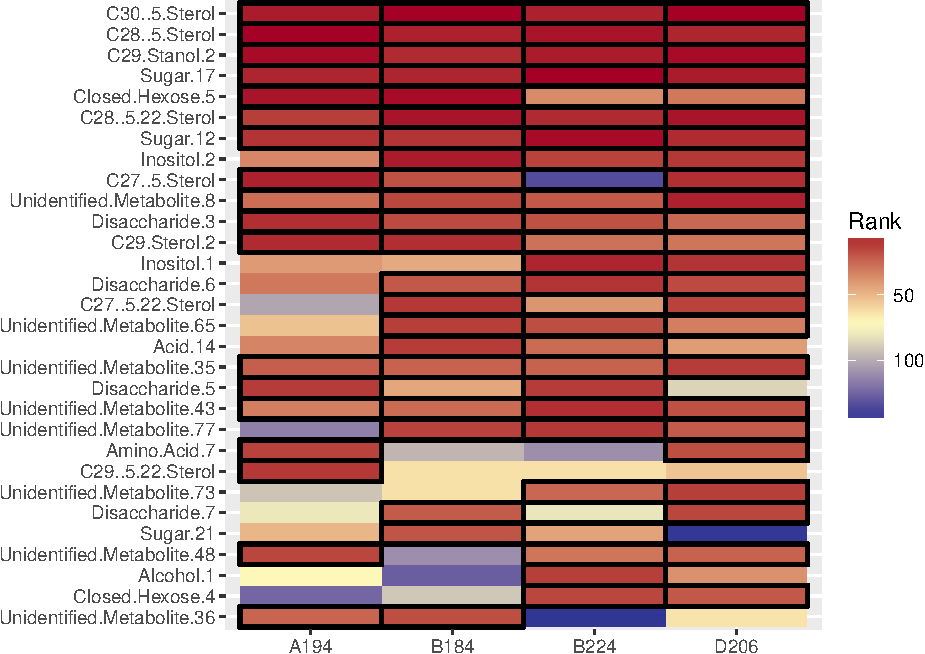
\includegraphics{rfPermute_ms_files/figure-latex/impHeatmap-1.pdf}
\caption{Heatmap of top 30 most important predictor metabolites, color
coded by rank order. Cells encircled by black have p-values \textless{}=
0.05.}
\end{figure}

\subsection{Model summary functions}\label{model-summary-functions}

\texttt{rfPermute} also provides a set of convenient summary functions
for \emph{randomForest} models, regardless of if the model was run in
\emph{randomForest} or \emph{rfPermute}. In order to evaluate how well a
classification model is performing, one should compare the observed OOB
error rates to what would be expected if samples were just randomly
allocated to bins in the absence of information from predictor
variables. This rate turns out to simply be the fraction of the total
sample size represented by each class. In a simple two-class model, with
equal sample sizes in each class, this is then 50\% for both classes.
However, if the sample sizes are skewed, say 80 in class A, and 10 in
class B, then one would expect on average to correctly classify 80 / 90
of the class A samples and 10 / 90 of the class B samples. Thus the
expected error rates would be 0.11 for class A and 0.89 for class B.
These values, referred to as ``priors'' are calculated by the
\texttt{exptdErrRate} function. Since this data set has equal sample
sizes, all priors are the same:

\begin{Shaded}
\begin{Highlighting}[]
\KeywordTok{exptdErrRate}\NormalTok{(metab.rf)}
\end{Highlighting}
\end{Shaded}

\begin{verbatim}
 OOB A194 B184 B224 D206 
0.75 0.75 0.75 0.75 0.75 
\end{verbatim}

The \texttt{classConfInt} function provides confidence intervals for the
class-specific and overall model classification scores based on a
binomial distribution. This helps provide a measure of uncertainty of
the true classification rate given the observed sample sizes.

\begin{Shaded}
\begin{Highlighting}[]
\KeywordTok{classConfInt}\NormalTok{(metab.rf)}
\end{Highlighting}
\end{Shaded}

\begin{verbatim}
        pct.correct  LCI_0.95  UCI_0.95 Pr.gt_0.8
A194        0.93750 0.6976793 0.9984189 0.9718525
B184        1.00000 0.7940928 1.0000000 1.0000000
B224        0.93750 0.6976793 0.9984189 0.9718525
D206        1.00000 0.7940928 1.0000000 1.0000000
Overall     0.96875 0.8916295 0.9961928 0.9999893
\end{verbatim}

The first column in the output is the oberved percent correct (1 - OOB
error rate). The next two columns are the bounds of the central
95-percentile of the classification score given the observed sample
sizes. The final column provides the fraction of the binomial
distribution that is greater than a given threshold. The default is 0.8,
but it can be specified using the \texttt{threshold} argument.

A complete summary of the \emph{randomForest} classification model can
be produced by combining the results of \texttt{classConfInt} and
\texttt{exptdErrRate} along with the full confusion matrix as in the
function, \texttt{confusionMatrix}.

\begin{Shaded}
\begin{Highlighting}[]
\KeywordTok{confusionMatrix}\NormalTok{(metab.rf)}
\end{Highlighting}
\end{Shaded}

\begin{verbatim}
        A194 B184 B224 D206 pct.correct LCI_0.95
A194      15    0    0    1      93.750 69.76793
B184       0   16    0    0     100.000 79.40928
B224       0    0   15    1      93.750 69.76793
D206       0    0    0   16     100.000 79.40928
Overall   NA   NA   NA   NA      96.875 89.16295
         UCI_0.95 Pr.gt_0.8 Prior
A194     99.84189  97.18525    25
B184    100.00000 100.00000    25
B224     99.84189  97.18525    25
D206    100.00000 100.00000    25
Overall  99.61928  99.99893    25
\end{verbatim}

Note that in this matrix, the columns deriving from the
\texttt{classConfInt} function are multiplied by 100, and \texttt{Prior}
is 100 * (1 - expected error rate), as I have found that this scale to
be more easily communicated in publications.

\subsection{Vote distributions}\label{vote-distributions}

When evaluating a Random Forest model, it can be useful to visualize the
distribution of votes for classes within the forest. From these
distributions, we can tell if individual cases are tending to be
correctly classified with large probabilities (have a high fraction of
trees voting for the correct class), or have equivocal assignments (vote
probabilities are roughly equal). We can also see if misclassified
samples were strongly or weakly misclassified. The \texttt{plotVotes}
function will produce such a distribution, either as a bar chart, which
is useful when few samples are present, or as an area chart, which is
more readable with many samples.

\begin{Shaded}
\begin{Highlighting}[]
\KeywordTok{plotVotes}\NormalTok{(metab.rf)}
\end{Highlighting}
\end{Shaded}

\begin{figure}[htbp]
\centering
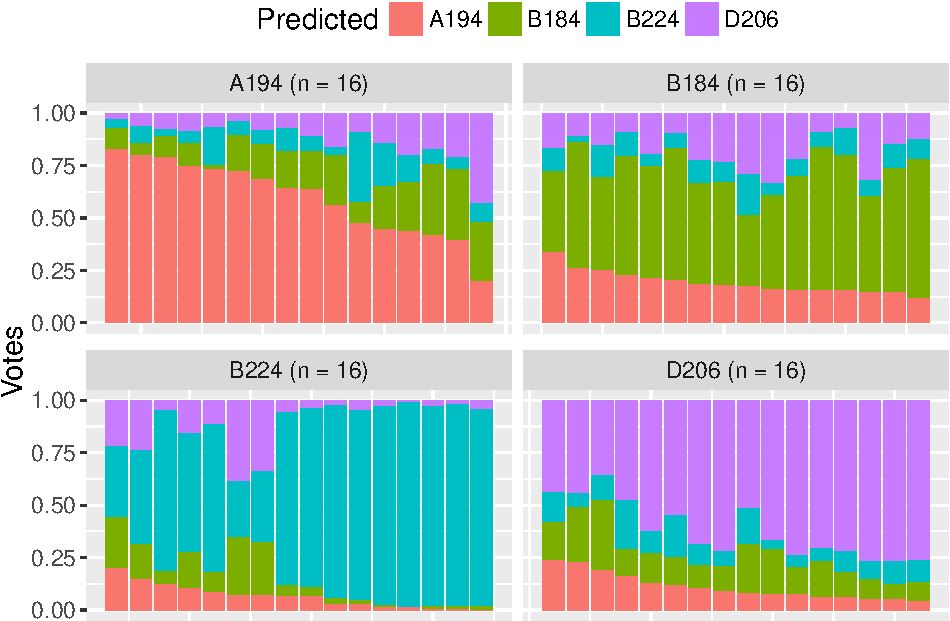
\includegraphics{rfPermute_ms_files/figure-latex/plotVotes-1.pdf}
\caption{Distribution of votes in the Random Forest for samples of each
of the four \emph{Symbiodinium} types.}
\end{figure}

Figure 5 shows that \emph{Symbiodinium} types A194 and D206 have many of
their members classified with a relatively large fraction of votes. We
also see that the two B224 samples that were misclassified to D206 only
had about 30\% of the votes to D206, which is not a strong
misclassification.

\subsection{Proximity plots}\label{proximity-plots}

For visualizing the relative distribution of samples in the Random
Forest, multi-dimensional scaling (MDS) is applied to the proxmity
matrix computed by \texttt{randomForest}. The \emph{randomForest}
package provides the \texttt{MDSplot} function which uses \emph{base}
graphics to visualize these points. In \emph{rfPermute} there is the
\texttt{proximityPlot} function which uses \emph{ggplot2} graphics
(Wickham 2009) and provides a few additional useful features. The result
of \texttt{proximityPlot} depicts the MDS projection of cases, with
classes encircled by a shaded convex hull. Additionally, each case is
represented by a color-coded dot and circle. The color of the interior
dot corresponds to the original case, while the color of the exterior
circle corresponds to the predicted case. Thus, correctly classified
cases will have the same color, while misclassified cases will have
different colors.

\begin{Shaded}
\begin{Highlighting}[]
\KeywordTok{proximityPlot}\NormalTok{(metab.rf)}
\end{Highlighting}
\end{Shaded}

\begin{figure}[htbp]
\centering
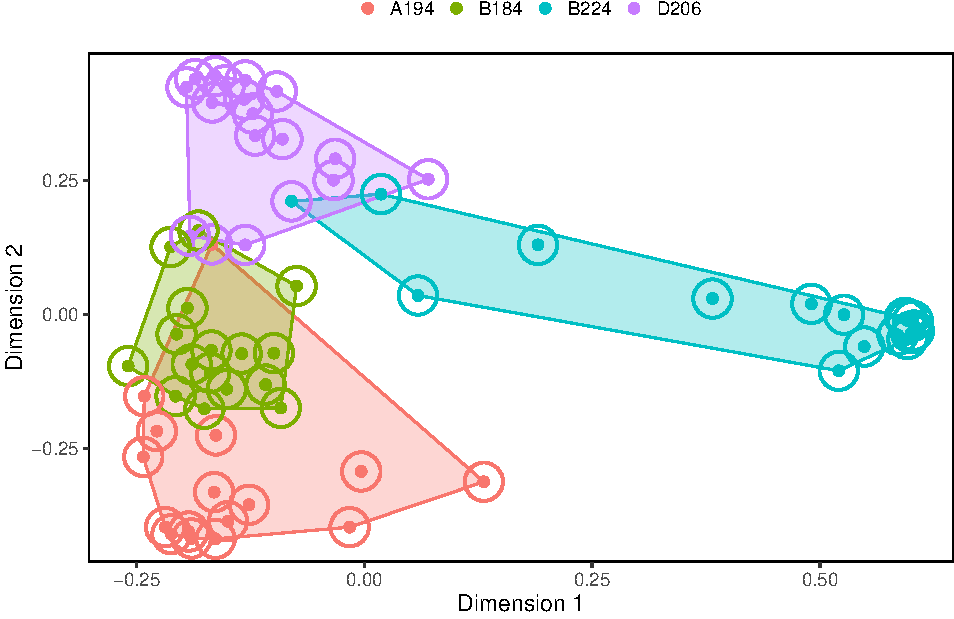
\includegraphics{rfPermute_ms_files/figure-latex/proximityPlot-1.pdf}
\caption{Proximity plot of \emph{Symbiodinium} samples.}
\end{figure}

In Figure 6, the two misclassified B224 samples are near the periphery
of the D206 convex hull, some distance away from the majority of the
other B224 samples, but also separated from the majority of the D206
samples. Given the variability in B224, we might then view these as
aberrant B224 samples rather than mislabelled D206 samples.

All graphical output in \emph{rfPermute} is produced using the
\emph{ggplot} package. Functions that produce figures will also
invisibly return the \emph{ggplot2} object generated so that they can be
further modified if desired. The \texttt{proximityPlot} function also
returns the MDS matrix resulting from a call to \texttt{cmdscale}.

\subsection{Performance}\label{performance}

Because the primary function, \texttt{rfPermute}, is a wrapper that
calls \texttt{randomForest} multiple times, execution time can be
lengthy for large data sets and will scale relatively linearly with the
number of permutations. However, execution time can be reduced if a
multi-core machine is used and the \texttt{num.cores} argument set
appropriately. For example, on a MacBook Pro with a 2.8GHz Intel Core i7
chip and 16GB of 1600 MHz DDR3 RAM, one \texttt{randomForest} run of the
\emph{Symbiodinium} data set took approximately 0.1 seconds. The same
\texttt{rfPermute} model with 100 replicates took 14.4 seconds, and 1000
replicates took 142.3 seconds. When the number of cores used was
increased from one to three, the 1000 replicate model took 46 seconds.

Efficiency can also be enhanced by running the same \emph{rfPermute}
model can on multiple systems and combining the results later using the
\texttt{rp.combine} function. This function is the equivalent of
\texttt{randomForest::combine} and takes a set of the same
\texttt{rfPermute} models as its arguments.

\subsection{Installation}\label{installation}

The stable version of \emph{rfPermute} can be installed from CRAN via:

\begin{Shaded}
\begin{Highlighting}[]
\KeywordTok{install.packages}\NormalTok{(}\StringTok{"rfPermute"}\NormalTok{)}
\end{Highlighting}
\end{Shaded}

To install the latest development version from GitHub, use:

\begin{Shaded}
\begin{Highlighting}[]
\CommentTok{# make sure you have Rtools installed}
\NormalTok{if (!}\KeywordTok{require}\NormalTok{(}\StringTok{"devtools"}\NormalTok{)) }\KeywordTok{install.packages}\NormalTok{(}\StringTok{"devtools"}\NormalTok{)}

\CommentTok{# install from GitHub}
\NormalTok{devtools::}\KeywordTok{install_github}\NormalTok{(}\StringTok{"EricArcher/rfPermute"}\NormalTok{)}
\end{Highlighting}
\end{Shaded}

\subsection*{References}\label{references}
\addcontentsline{toc}{subsection}{References}

\hypertarget{refs}{}
\hypertarget{ref-RN125}{}
Berk, R. 2006. ``An Introduction to Ensemble Methods for Data
Analysis.'' Journal Article. \emph{Sociological Methods and Research} 34
(3): 263--95.

\hypertarget{ref-RN266}{}
Breiman, L. 2001. ``Random Forests.'' Journal Article. \emph{Machine
Learning} 45 (1): 5--32.

\hypertarget{ref-RN403}{}
---------. 2002. ``Manual on Setting up, Using, and Understanding Random
Forests V3.1.'' Journal Article.
\url{http://oz.berkeley.edu/users/breiman/Using_random_forests_V3.1.pdf}.

\hypertarget{ref-RN126}{}
Cutler, D. R., T.C. Jr. Edwards, K. H. Beard, A Cutler, K.T. Hess, J.
Gibson, and J.J. Lawler. 2007. ``Random Forests for Classification in
Ecology.'' Journal Article. \emph{Ecology} 88 (11): 2783--92.

\hypertarget{ref-RN127}{}
Liaw, A., and M. Wiener. 2002. ``Classification and Regression by
RandomForest.'' Journal Article. \emph{R News} 2/3: 18--22.

\hypertarget{ref-RN128}{}
Touw, W.G., J.R. Bayjanov, L Overmars, L Backus, J Boekhorst, M Wels,
and S. A. F. T. van Hijum. 2012. ``Data Mining in the Life Sciences with
Random Forest: A Walk in the Park or Lost in the Jungle?'' Journal
Article. \emph{Briefings in Bioinformatics} 14 (3): 316--26.
doi:\href{https://doi.org/10.1093/bib/bbs034}{10.1093/bib/bbs034}.

\hypertarget{ref-Wickham2009}{}
Wickham, Hadley. 2009. \emph{Ggplot2: Elegant Graphics for Data
Analysis}. Springer-Verlag New York. \url{http://ggplot2.org}.

\hypertarget{ref-RN268}{}
Winham, S.J., C.L. Colby, R.R. Freimuth, X. Wang, M. de Andrade, M.
Huebner, and J.M. Biernacka. 2012. ``SNP Interaction Detection with
Random Forests in High-Dimensional Genetic Data.'' Journal Article.
\emph{BMC Bioinformatics} 13: 164.

\end{document}
